\section{Connecting to the PCDB}\label{sec_connecting_to_the_PCDB}

After opening \texttt{pgAdmin3}, click `Add Server...' in the `File' tab of the program's menu bar, or click the toolbar icon looking like a plug; see figure \ref{fig_pgadmin3_add_server}).

\begin{figure}[h!]
\centering
  \begin{subfigure}{.45\textwidth}
  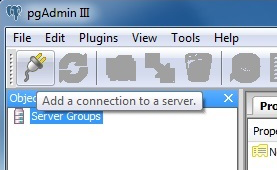
\includegraphics[width=\textwidth,trim= 0 0 0 0, clip]{pcdb_documentation_screenshots/pgadmin3_add_server.png}
    \subcaption{Click on plug icon to open `New Server Registration' interface.}
    \label{fig_pgadmin3_add_server}
  \end{subfigure}
  ~%
  \begin{subfigure}{.45\textwidth}
  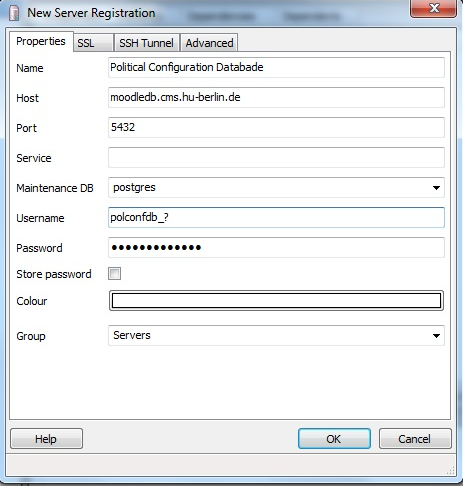
\includegraphics[width=\textwidth,trim= 0 0 0 0, clip]{pcdb_documentation_screenshots/pgadmin3_new_server_registration.png}
    \subcaption{Enter server information to `New Server Registration' interface.}
    \label{fig_pgadmin3_server_registration}
  \end{subfigure} 
  \caption{How to add and register a new server connection in \texttt{pgAdmin3}.}
\end{figure}

Enter the following properties of the PCDB in the corresponding lines of the Properties-tab of \texttt{pgAdmin3}'s `New Server Registration' wizard (see figure \ref{fig_pgadmin3_server_registration}):\\
\begin{itemize}
%Databasesysteme & \texttt{\footnotesize PostgreSQL} \\
\item[]{{\bf Name}: {\em Choose a name for the server connection!} (\texttt{\footnotesize Political Configuration Database} or \texttt{\footnotesize CMS Database} recomended)}
\item[]{{\bf Host}: \texttt{\footnotesize moodledb.cms.hu-berlin.de} }
\item[]{{\bf Port}: \texttt{\footnotesize 5432} }
%\item[]{{\bf SSL-Port}: \texttt{\footnotesize 5432} }
\item[]{{\bf Maintenance DB}: \texttt{\footnotesize postgres} }
\item[]{{\bf Username \& Password}: Contact \href{mailto:tarik.abou-chadi@hu-berlin.de}{the administrator} to receive a username and a user password! }
\end{itemize}
Please always unselect the `Store password' checkbox for security reasons! Finally, click `OK' to connect to the server.

\paragraph{In case you fail}
In case \texttt{pgAdmin3} prompts an error message on your server connection attempt in the `New Server Registration' wizar, read through carefully the error message and alos double-check your input (its likely that the error is due to a spelling error in your input). 
Always do some online research first (e.g., search the error message in Google or browse \texttt{pgAdmin3}'s documentation under \url{https://www.pgadmin.org/docs/dev/index.html}) in order to fix your problems. 

Should you not be able to fix your problem, and hence unablt to connect to the CMS database server, you can contact the CMS database service via email: \href{mailto:dbtech@cms.hu-berlin.de}{dbtech@cms.hu-berlin.de}
In case it turns out to be an issue with your version of \texttt{pgAdmin3}, contact your IT team (in the ISW this is Andreas Goroncy, \href{mailto:andreas.goroncy@sowi.hu-berlin.de}{andreas.goroncy@sowi.hu-berlin.de} or phone (030)~2093~4389).


\paragraph{In case you succeed}
Once you have successfully connected to the CMS database server, an element with the name you gave your server connection in the registration will appear in the `Object browser' (left panel below toolbar in \texttt{pgAdmin3}).  
Double-click on this icon to access the server. 

\begin{figure}[ht!]
\centering
  \begin{subfigure}{.45\textwidth}
  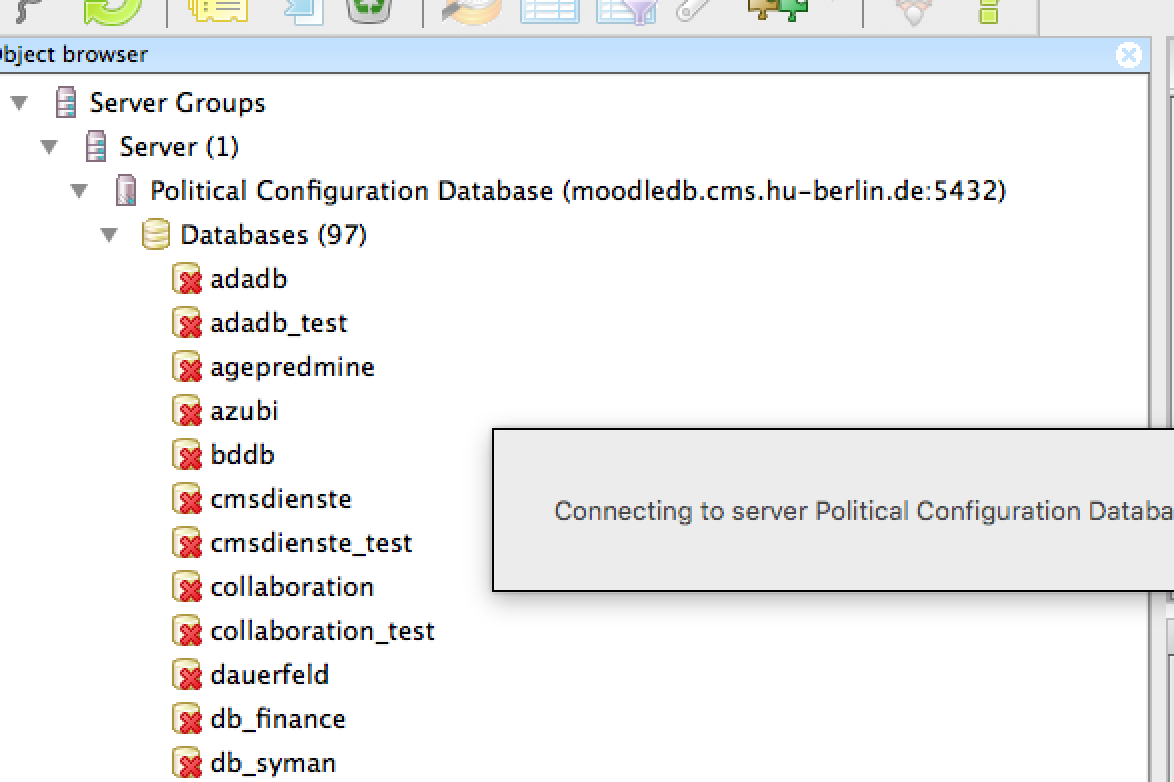
\includegraphics[width=\textwidth,trim= 0 0 0 0, clip]{pcdb_documentation_screenshots/pgadmin3_databases_on_server.png}
    \subcaption{View of `Object browser' window after connecting to the CMS database server.}
    \label{fig_pgadmin3_databases_on_server}
  \end{subfigure}
  ~%
  \begin{subfigure}{.45\textwidth}
  \includegraphics[width=\textwidth,trim= 0 0 0 0, clip]{pcdb_documentation_screenshots/pgadmin3_inside_pcdb.png}
    \subcaption{Inside the \texttt{polconfdb} database (PCDB) in the `Object browser' window.}
    \label{fig_pgadmin3_inside_pcdb}
  \end{subfigure} 
  \caption{Connecting to the CMS database server and accessing the PCDB in \texttt{pgAdmin3}.}
\end{figure}

Several databases will be associated in the `Object browser' with your server connection (see figure \ref{fig_pgadmin3_databases_on_server}).
The only database that is open to your access though is named \texttt{\footnotesize polconfdb} (see figure \ref{fig_pgadmin3_inside_pcdb}). (In contrast to the other databases, its icon is not visually marked with a red cross.) 

By default, to the right of the `Object browser' panel, you should see an information panel (upper-right, see figure \ref{fig_pgadmin3_inside_pcdb_information_panel}), and a `SQL pane' (lower-right panel, see figure \ref{fig_pgadmin3_inside_pcdb_SQL_pane}). 
The information panel always informs you about the properties, statistics, etc. of the object you have currently selected in the `Object browser,' and the `SQL pane' displays the definition of this object in SQL.

\begin{figure}[ht!]
\centering
  \begin{subfigure}{.45\textwidth}
  \includegraphics[width=\textwidth,trim= 0 0 0 0, clip]{pcdb_documentation_screenshots/pgadmin3_inside_pcdb_information_panel.png}
    \subcaption{View of `Object browser' window after connecting to the CMS database server.}
    \label{fig_pgadmin3_inside_pcdb_information_panel}
  \end{subfigure}
  ~%
  \begin{subfigure}{.45\textwidth}
  \includegraphics[width=\textwidth,trim= 0 0 0 0, clip]{pcdb_documentation_screenshots/pgadmin3_inside_pcdb_SQL_pane.png}
    \subcaption{`SQL pane' display for \texttt{polconfdb} database (PCDB).}
    \label{fig_pgadmin3_inside_pcdb_SQL_pane}
  \end{subfigure} 
  \caption{Information and SQL panels of the \texttt{polconfdb} database in \texttt{pgAdmin3}.}
\end{figure}
